%%%%%%%%%%%%%%%%%%%%%%%%%%%%%%%%%%%%%%%%%%%%%%%%%%%%%%%%%%%%%%%%%%%%%%%%%%%%%%%%
%              Capitulo 4: Arquitectura general del sistema                    %
%%%%%%%%%%%%%%%%%%%%%%%%%%%%%%%%%%%%%%%%%%%%%%%%%%%%%%%%%%%%%%%%%%%%%%%%%%%%%%%%

\chapter{Arquitectura general del sistema}
\label{chap:arch}

El objetivo del sistema es, dados un archivo que contiene un dominio de planificación \texttt{PDDL}
que describe un determinado juego y un archivo de configuración que especifica una serie de parámetros
del sistema, resolver un nivel de dicho juego generando los problemas de planificación
\texttt{PDDL} hasta los objetivos especificados de forma automática a partir de los estados de observación
del juego.

Este sistema está estructurado en una serie de módulos lógicos que representan una
tarea de alto nivel. Un módulo lógico se compone a su vez de diversos módulos
funcionales o procesos, los cuales llevan a cabo una tarea concreta y se comunican con
otros módulos funcionales del mismo módulo lógico para llevar a cabo dicha tarea de alto
nivel.

La tarea que un módulo funcional lleva a cabo puede realizarse de forma automática o
puede llegar a requerir de la interacción con el usuario para poder ser completada.
Cabe destacar además que, en determinados casos, los módulos funcionales de un módulo
lógico pueden comunicarse con los módulos funcionales de otros módulos lógicos, lo cual se
describirá más detenidamente más adelante.

Por lo pronto, los módulos lógicos principales que se han considerado a la hora de definir
la arquitectura son los siguientes:

\begin{itemize}[label=\textbullet]
    \item Un módulo de interacción con el usuario (\textit{User interaction}).
    \item Un módulo de planificación (\textit{Planning}).
    \item Un módulo de monitorización y ejecución del plan (\textit{Plan Execution \& Monitoring}).
\end{itemize}

En la figura \ref{fig:system_arch} pueden verse los distintos módulos lógicos y funcionales que
componen el sistema, además de cómo están organizados, cómo se comunican y qué información se
envían entre ellos.

\begin{figure}[H]
    \centering
    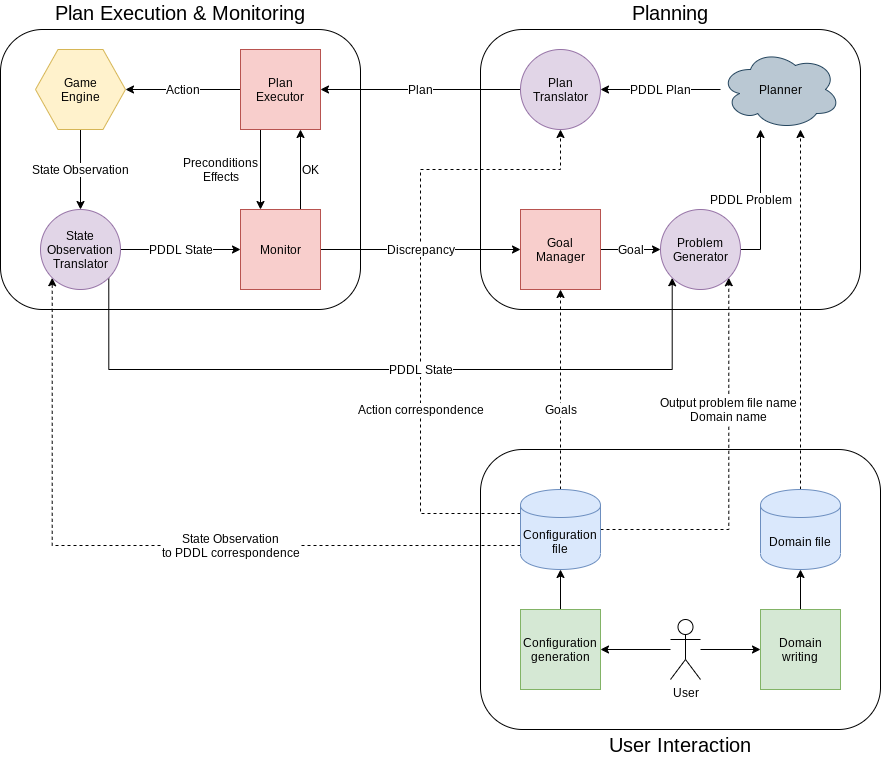
\includegraphics[scale=0.4]{img/CH04/system_arch.png}
    \caption{Esquema de la arquitectura general del sistema.}
    \label{fig:system_arch}
\end{figure}

Tomando en consideración dicho esquema, vamos a comentar brevemente cual es
la funcionalidad básica de cada módulo lógico y cómo interactúan entre ellos.
En el próximo capítulo desglosaremos cada uno de ellos y estudiaremos los módulos
funcionales que los componen, de forma que se obtendrá una mejor visión de cómo
funciona cada componente y de cómo interactúa con las demás.

Empecemos por la parte fundamental, la cual es el \textbf{módulo de interacción con el usuario}
(\textit{User Interaction}). Como se puede suponer y por lo que se ha comentado anteriormente,
este es el módulo menos automatizado, ya que es con el que interactúa directamente el usuario.
Es aquí donde se encuentran dos de los procesos más importantes: la creación del dominio
(\textit{Domain writing}) y la creación del archivo de configuración
(\textit{Configuration generation}) que utilizará el sistema.

Por una parte, el usuario tiene que definir el dominio de planificación \texttt{PDDL}. Este dominio está
compuesto por una serie de predicados y tipos de objetos que intentan modelar el
juego (por ejemplo conexiones entre casillas, objetos del juego, información sobre la
posición de los elementos, etc.). También forman parte del dominio una serie de acciones
que, con sus precondiciones y efectos, pretenden reflejar las acciones del juego. No obstante,
también se pueden tener otras acciones que no tengan ningún tipo de correspondencia, las cuales
podrían considerarse accione auxiliares. Como se puede suponer, el sistema tendrá que traducir
el estado del juego para adaptarse a la representación en formato \texttt{PDDL} que ha
creado el usuario.

Por otra parte, el usuario debe especificar una serie de parámetros en el archivo de
configuración que se utilizarán en el sistema para realizar una serie de tareas.
Entre dichas tareas se incluyen:

\begin{itemize}[label=\textbullet]
    \item La traducción de estados de observación del juego a estados \texttt{PDDL}
    (\textit{State Observation Translation}) mediante una serie de correspondencias entre
    los elementos de los estados de observación (obtenidos automáticamente del \textit{GVGAI Engine})
    y predicados \texttt{PDDL} (\textit{State Observation to \texttt{PDDL} correspondence}).
    \item La traducción de acciones \texttt{PDDL} a acciones de \texttt{GVGAI}
    (\textit{Plan Translator}) mediante una serie de correspondencias entre las acciones de
    \texttt{PDDL} y las de \texttt{GVGAI} (\textit{Action correspondence}).
    \item La gestión de los objetivos (\textit{Goal Manager}) teniendo en cuenta los
    objetivos proporcionados por el usuario (\textit{Goals}).
    \item La generación de los problemas \texttt{PDDL} (\textit{Problem Generator})
    especificando el nombre del fichero de problema de salida (\textit{Output problem file name})
    y el nombre del dominio (\textit{Domain name}).
\end{itemize}


Otro módulo lógico que se encuentra en el sistema es el \textbf{módulo de planificación}
(\textit{Planning}). Este módulo se encarga de gestionar los objetivos (\textit{Goals}) cuando
sea necesario, estableciendo el objetivo actual y determinando cuales se han cumplido y cuales no
(\textit{Goal Manager}). También es el módulo responsable de generar un archivo de problema
(\textit{Problem Generator}), de obtener un plan válido hasta un predicado objetivo dado
(\textit{Planner}) y de traducir posteriormente dicho plan para que pueda ser ejecutado
en el entorno de juego (\textit{Plan Translator}).

Por último tenemos el \textbf{módulo de ejecución del plan y de monitorización}
(\textit{Plan Execution \& Monitoring}). Como su propio nombre indica, este módulo
se encarga de ejecutar el plan obtenido por el módulo de planificación (\textit{Plan Executor})
y de monitorizar dicha ejecución (\textit{Monitoring}), determinando en el proceso si se ha
producido alguna discrepancia, y si por tanto hace falta replanificar. Una \textbf{\textit{discrepancia}} implica
que se ha producido un cambio en el estado del juego que no se esperaba a la hora de obtener
el plan original, y por tanto éste ha dejado de ser válido y hace falta encontrar uno nuevo.
En el proceso de comprobar si se ha producido una discrepancia se tiene que realizar la traducción del
estado de observación del juego a predicados \texttt{PDDL} (\textit{State Observation Translator}),
ya que esta información se utiliza por el monitor para estudiar la existencia de discrepancias.
Para ejecutar el plan se mandan las acciones al motor del juego (\textit{Game Engine}), el cual
se encargará de procesarlas de la forma adecuada.

En cuanto a las interacciones entre los módulos, el módulo de ejecución del plan y de
monitorización y el de planificación interactúan directamente entre ellos. El primero
comunica al segundo si se ha producido alguna discrepancia, y el segundo debe determinar
un nuevo objetivo y encontrar un plan hasta dicho objetivo. Posteriormente, el plan obtenido
es comunicado al primer módulo, el cual se encargará de hacer las operaciones pertinentes
con él.

El módulo de interacción con el usuario se comporta como un proveedor con los otros dos
módulos, ya que les proporciona la información necesaria para que éstos puedan
llevar a cabo ciertas tareas. Al funcionar como un proveedor, la comunicación es unilateral,
ya que no obtiene ningún tipo de respuesta de ellos.
